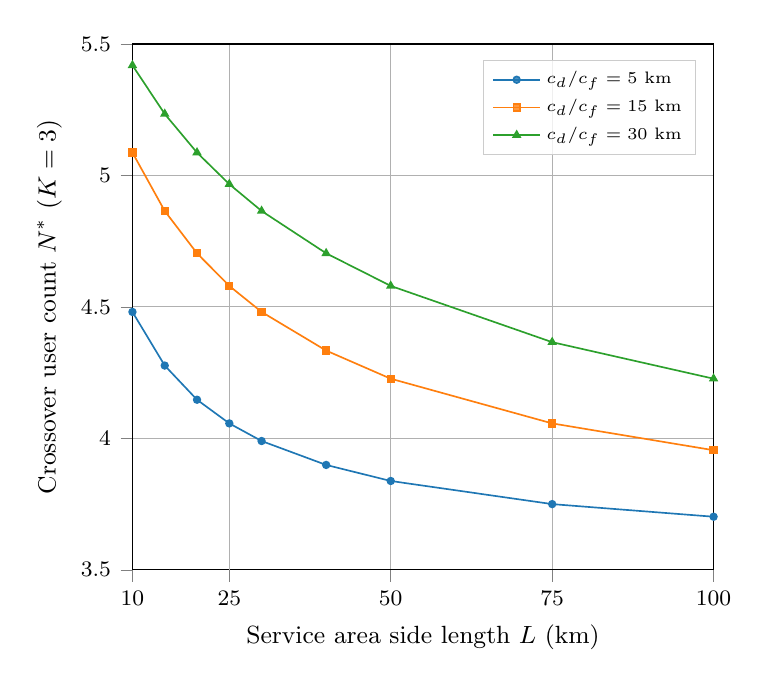
\begin{tikzpicture}

\definecolor{darkgray176}{RGB}{176,176,176}
\definecolor{lightgray204}{RGB}{204,204,204}
\definecolor{steelblue31119180}{RGB}{31,119,180}
\definecolor{darkorange25512714}{RGB}{255,127,14}
\definecolor{forestgreen4416044}{RGB}{44,160,44}

\begin{axis}[
width=210pt,
height=190pt,
scale only axis,
tick label style={font=\fontsize{8}{10}\selectfont},
label style={font=\fontsize{9}{11}\selectfont},
legend cell align={left},
legend style={
  fill opacity=0.8,
  draw opacity=1,
  text opacity=1,
  at={(0.97,0.97)},
  anchor=north east,
  draw=lightgray204,
  font=\fontsize{6}{8}\selectfont
},
tick align=outside,
tick pos=left,
x grid style={darkgray176},
xlabel={Service area side length $L$ (km)},
xmajorgrids,
xmin=10, xmax=100,
xtick={10,25,50,75,100},
y grid style={darkgray176},
ylabel={Crossover user count $N^*$ ($K=3$)},
ymajorgrids,
ymin=3.5, ymax=5.5,
ytick={3.5,4,4.5,5,5.5},
]

\addplot [semithick, steelblue31119180, mark=*, mark size=1.2, mark options={solid}]
table {%
10 4.481
15 4.277
20 4.147
25 4.057
30 3.990
40 3.899
50 3.838
75 3.750
100 3.702
};
\addlegendentry{$c_d/c_f=5$~km}
\addplot [semithick, darkorange25512714, mark=square*, mark size=1.2, mark options={solid}]
table {%
10 5.087
15 4.865
20 4.704
25 4.580
30 4.481
40 4.334
50 4.227
75 4.057
100 3.955
};
\addlegendentry{$c_d/c_f=15$~km}
\addplot [semithick, forestgreen4416044, mark=triangle*, mark size=1.4, mark options={solid}]
table {%
10 5.419
15 5.234
20 5.087
25 4.967
30 4.865
40 4.704
50 4.580
75 4.366
100 4.227
};
\addlegendentry{$c_d/c_f=30$~km}

\draw [dashed, darkgray176] (axis cs:25,3.5) -- (axis cs:25,5.5);

\end{axis}
\end{tikzpicture}
